\section{Nominal algorithm}
\label{sec:nominal}

Nominal algorithm and performance.

\begin{figure}[!htpb]
  \begin{center}
    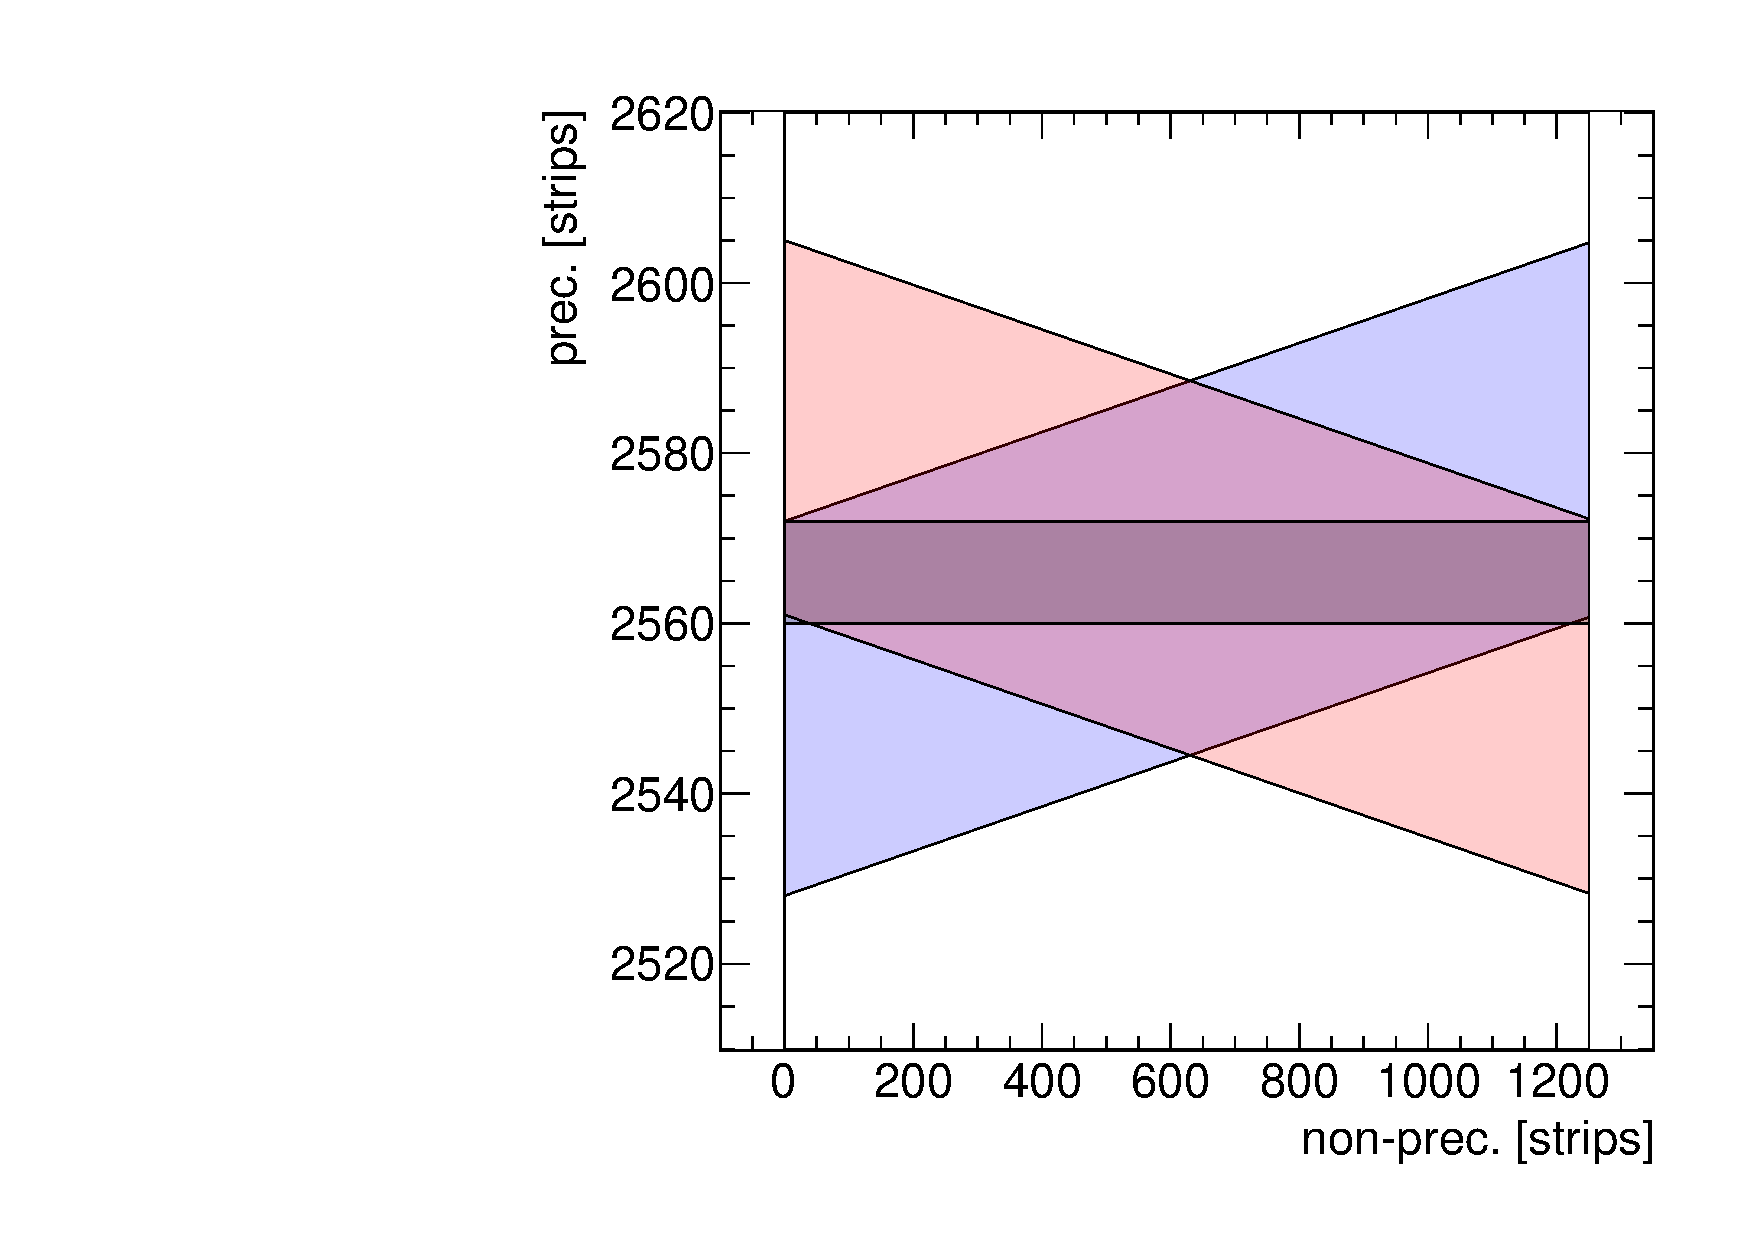
\includegraphics[width=0.48\textwidth]{figures/cartoon_roads_small_nominal.pdf}
    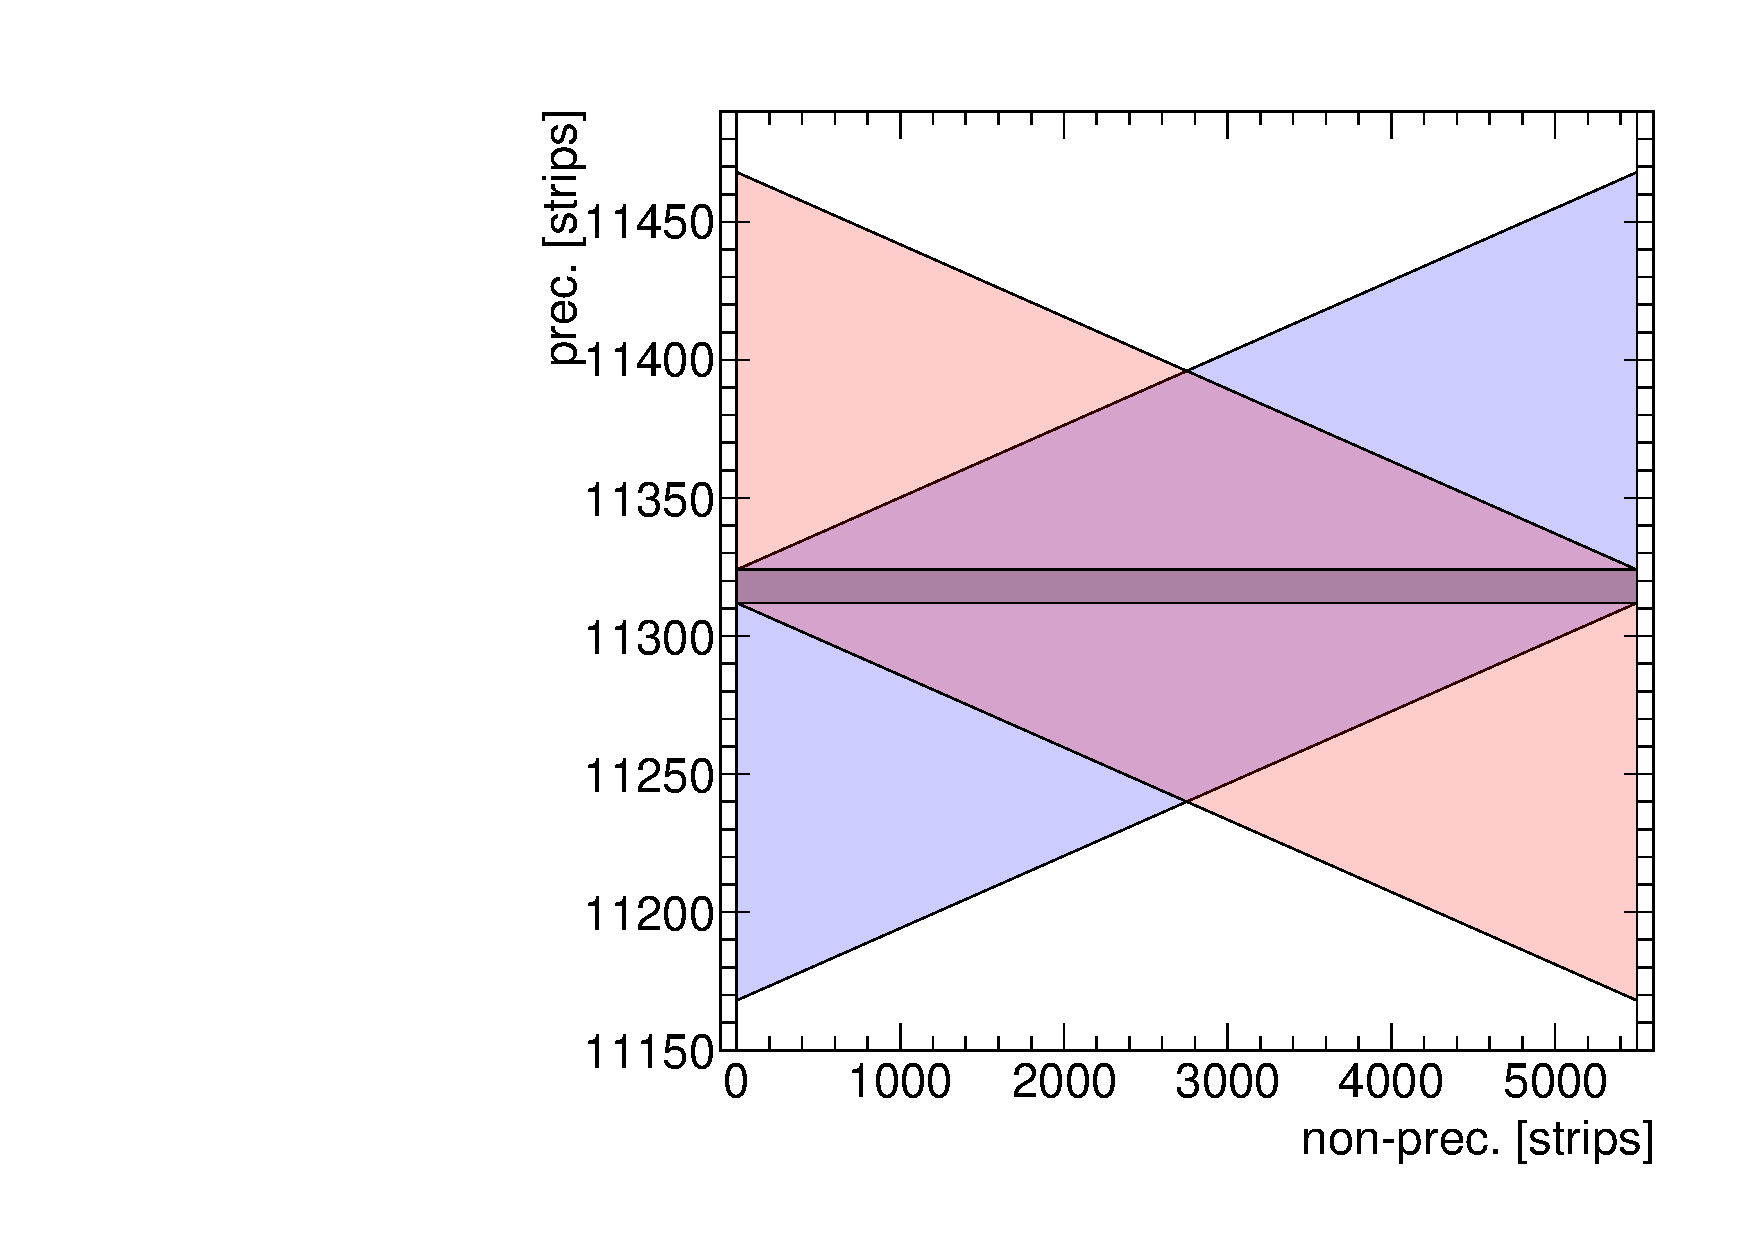
\includegraphics[width=0.48\textwidth]{figures/cartoon_roads_large_nominal.pdf}
  \end{center}
  \vspace{-10pt}
  \caption{Sketch of the road coverage of the nominal MMTP algorithm, for a small chamber closest to the beamline (left) and large chamber farthest from the beamline (right). The $X$ road is horizontal, the $U$ road is pink and slanted, and the $V$ road is blue and slanted. The x-axis and y-axis are in units of strip pitches, which are 0.4 mm.}
  \label{fig:cartoon_nominal}
\end{figure}

\begin{figure}[!htpb]
  \begin{center}
    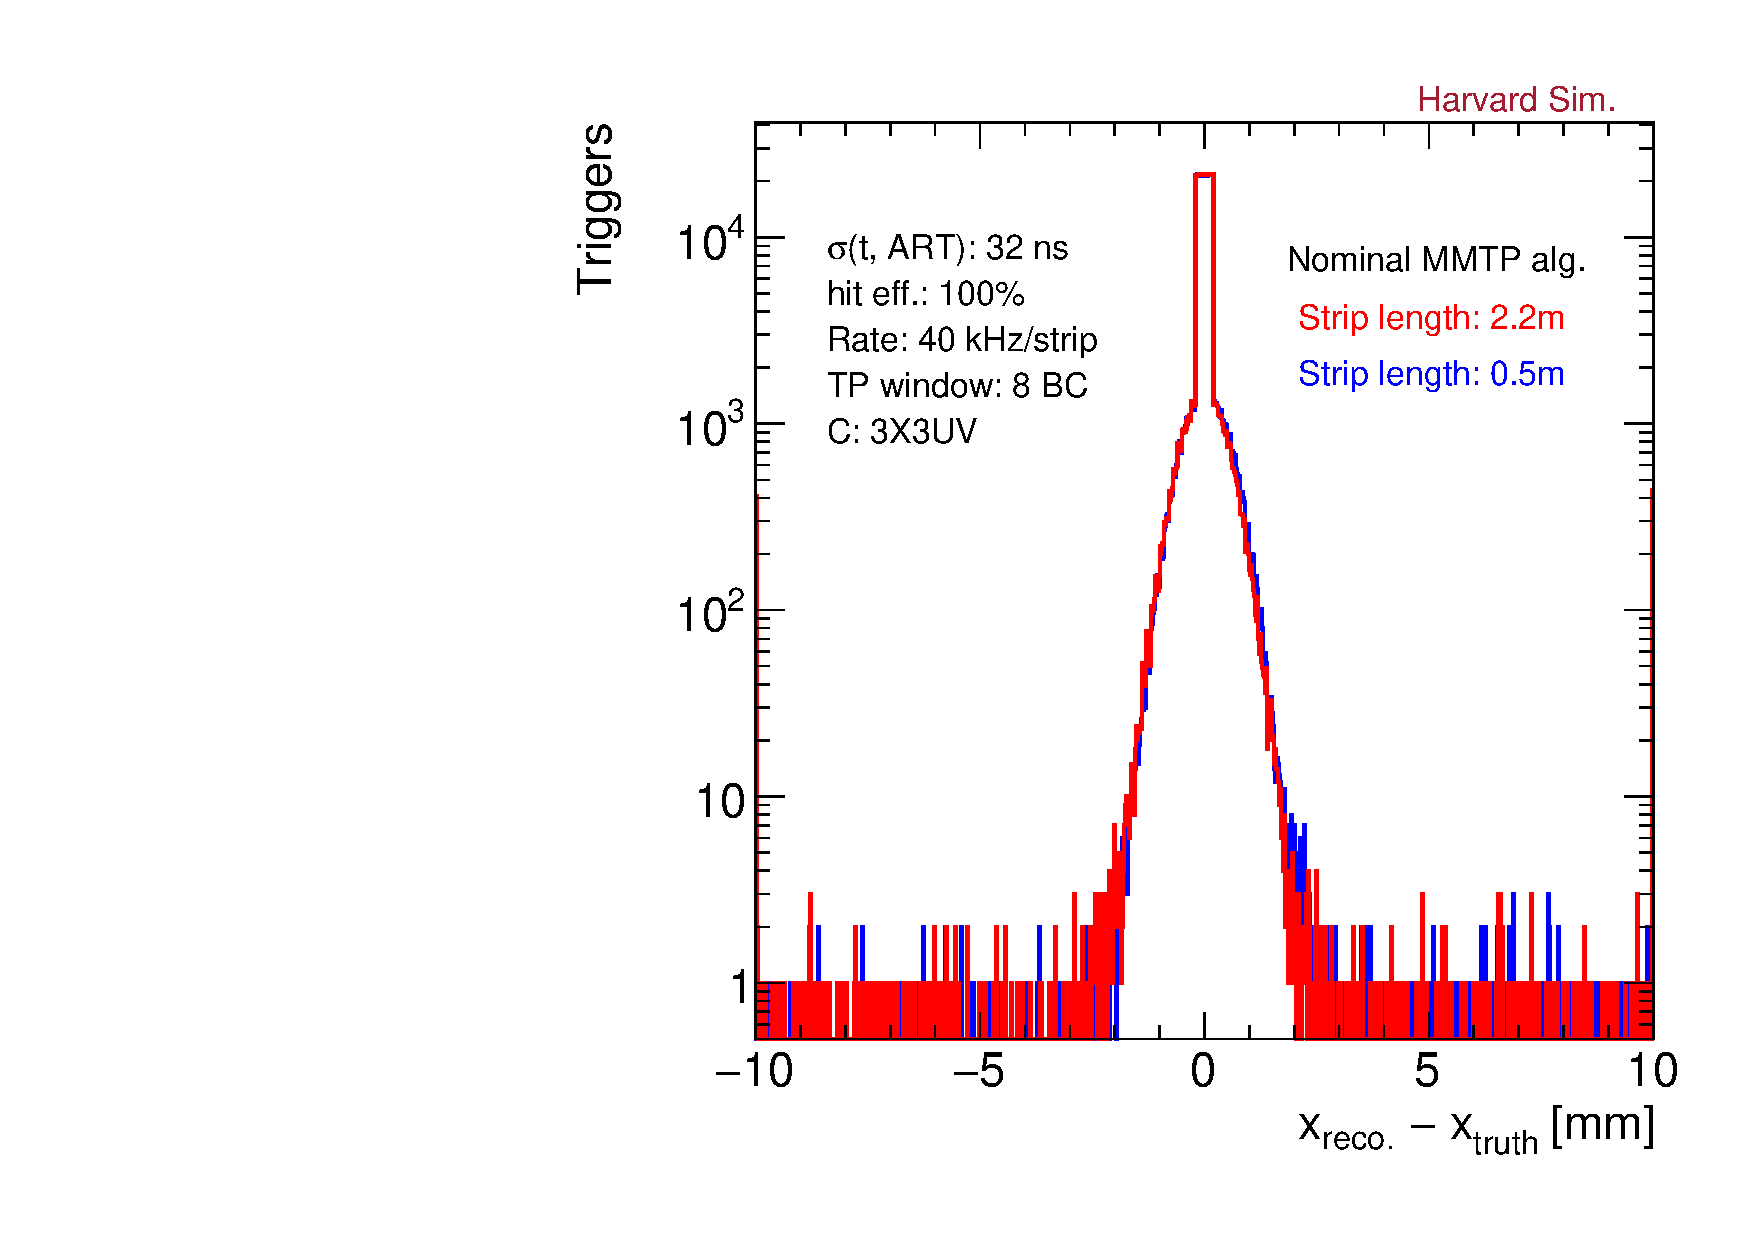
\includegraphics[width=0.48\textwidth]{figures/xres_old.pdf}
    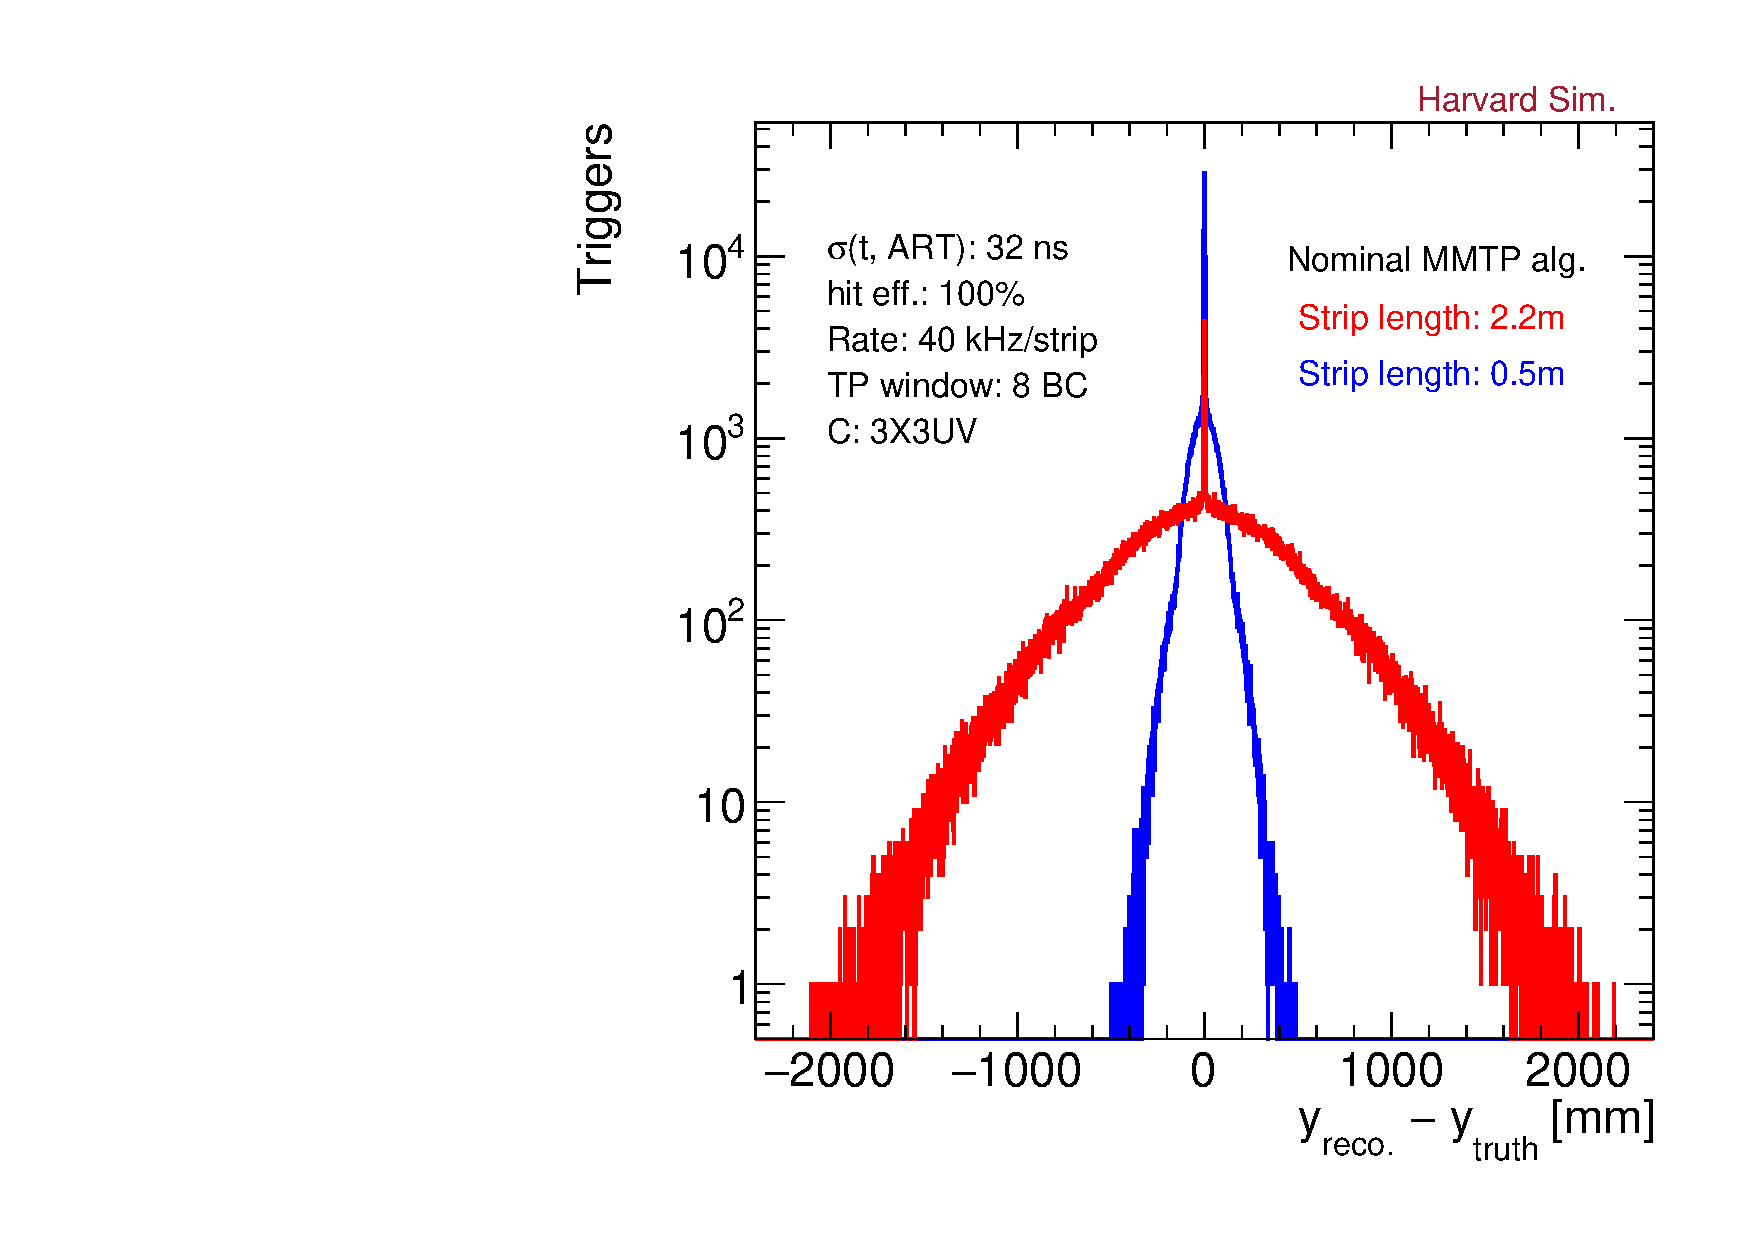
\includegraphics[width=0.48\textwidth]{figures/yres_old.pdf}
    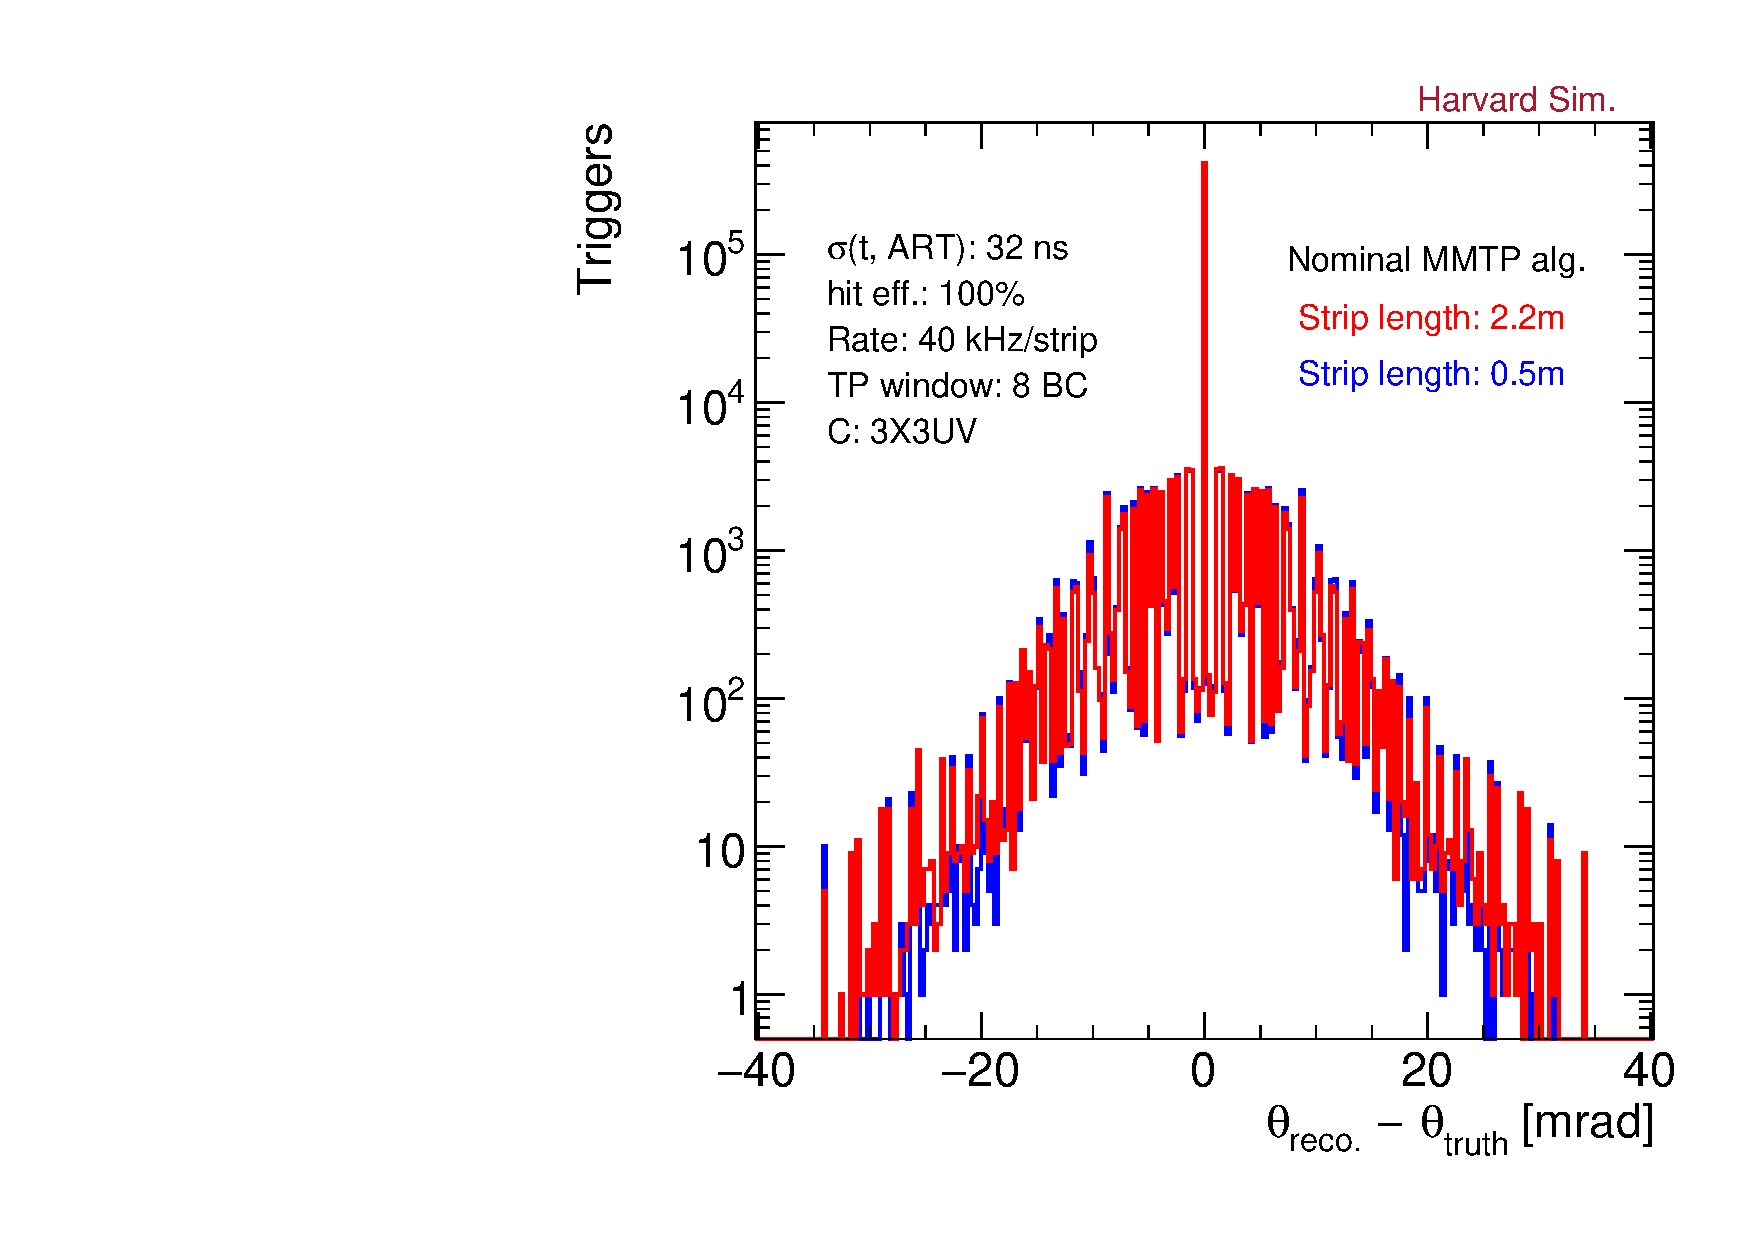
\includegraphics[width=0.48\textwidth]{figures/mres_old.pdf}
  \end{center}
  \vspace{-10pt}
  \caption{Distribution of $x_\text{reco.} - x_\text{truth}$ (top, left), $y_\text{reco.} - y_\text{truth}$ (top, right) and $\theta_\text{reco.} - \theta_\text{truth}$ (bottom) for the nominal MMTP algorithm with uncorrelated background at a rate of 40 kHz per strip.}
  \label{fig:resolutions_old}
\end{figure}
